\documentclass[11pt,a4paper]{article}
\usepackage{cmap}
\usepackage[utf8]{inputenc}
\usepackage[german]{babel}
\usepackage[left=1.5cm,right=1.5cm,top=1.5cm,bottom=1.5cm]{geometry}
\author{Andreas Hemmetter}
\let\footruleskip\undefined %undefine footruleskip
\usepackage{fancyhdr}
\usepackage{multicol}
\usepackage{microtype}
% \usepackage{textcomp}
% \usepackage{amsthm}
\usepackage{framed}
\usepackage{multirow}
\usepackage{xhfill}
\usepackage{makecell}
% \usepackage{bbold}
% \usepackage{amssymb}
\usepackage{hyperref}
\usepackage{booktabs}
\usepackage{graphicx}
\usepackage{setspace}
\usepackage{lettrine}
%\usepackage{braket}
% \usepackage{tikz}
% \usetikzlibrary{arrows}
\usepackage[sorting=none]{biblatex}
\addbibresource{refs.bib}
\AtBeginBibliography{\small} 
\definecolor{shadecolor}{rgb}{0.95, 0.95, 0.95}

\setlength{\headheight}{15.2pt}
\begin{document}
\pagestyle{fancyplain}
\fancyhf{}
\rhead{\textbf{\textit{Weltföderation}} - \href{mailto:ahemmetter@gmail.com}{A. Hemmetter} }
\rfoot{\scriptsize{ \href{https://creativecommons.org/licenses/by-sa/4.0/}{Creative Commons Namensnennung - Weitergabe unter gleichen Bedingungen 4.0 International Lizenz}}}
\begin{center}

\begin{tabular}[t]{@{}l}
\rule[4pt]{0.29\linewidth}{4pt}
\end{tabular}
\begin{tabular}[t]{@{}}
\fontsize{24pt}{10pt}
\textbf{Weltföderation}
\end{tabular}
\begin{tabular}[t]{r@{}}
\rule[4pt]{0.29\linewidth}{4pt}
\end{tabular}
\end{center}

\begin{multicols}{2}
\lettrine[lraise=0.1, lines=2]{\textsc{M}}{enschen} arbeiten seit über 12 000 Jahren an unserer Zivilisation. Durch Wissenschaft, Kunst, Philosophie, Technologie und harter Arbeit haben wir uns in eine gänzlich neue Welt katapultiert. Doch unsere politischen Einrichtungen haben bisher nicht aufgeholt: wir sind immer noch in den Strukturen der letzten Jahrhunderte gefangen.

\noindent Die Welt ist heute ein globales Dorf. Reisen, das Internet, Märkte und die Natur weben ein immer engeres Netz um uns Menschen. In dieser zusammenhängenden Welt sind Nationen zu klein geworden, als dass sie zur Lösung unserer wichtigsten Probleme etwas beitragen könnten. Eine demokratisch gewählte Regierung einer Weltföderation ist der beste Versuch, um uns selbst zu retten und unser Potential freizusetzen.


\begin{shaded*}
\noindent \textit{Bis die Fahnen still sich senkten,\\
bis die Trommel ausgegellt\\
\noindent in dem Parlament der Menschheit, \\
auf dem Bundestag der Welt.}
%\vspace{-22pt}
\begin{flushright}
-- Alfred Tennyson
\end{flushright}
\vspace{-12pt}
\end{shaded*}


\paragraph{Eine Gesichte der Vereinigung}

Unserer kollektiven Geschichte ist eine von kontinuierlicher Vereinigung. Von den Stämmen in der Steinzeit bis zur Gründung moderner Nationalstaaten haben sich unsere Vorväter stets mit ehemaligen Feinden in größeren Ländern zusammengeschlossen. Sie haben Recht und Ordnung formuliert, interpretiert und durchgesetzt, um Frieden, Wohlstand und Fortschritt im Angesicht wachsender Probleme zu sichern.\\
\noindent Frieden ist nicht nur die Abwesenheit von Krieg, sondern vielmehr die Konfliktlösung durch Recht und Gesetz. Tagtäglich führen unsere Staaten, Länder, Kreise, Gemeinden und Familien diese Pflicht unablässig aus. Gesetze, zusammen mit Feuer, dem Rad, Schrift und Elektrizität haben sich als die erfolgreichsten Erfindungen der Menschheit herausgestellt. Wenn du Frieden willst, bereite das Gesetz vor.

\noindent Interessanterweise tritt dieses allgemeingültige Prinzip auf der Weltbühne hinter den Götzen der nationalstaatlichen Selbstbestimmung. Folgende Wahrheit halten wir als selbstverständlich: dass mein Staat absolute Freiheit besitzt, seine Interessen zu verteidigen. Wer verteidigt die Interessen der Menschheit?

\end{multicols}
\paragraph{Not macht an keiner Grenze halt}

Die Welt hat sich verändert. Probleme sind nicht mehr klein genug, um von einzelnen Ländern gelöst zu werden. Die Bedrohungen, die uns gegenüberstehen, haben keinen Respekt für Grenzen.\\
\noindent Jeder atmet die gleiche Atmosphäre.
Treibhausgase verändern unser Klima, egal wo am meisten ausgestoßen wurde.
Obwohl wir die Lösungen kennen, sind die Staaten in ihrem Wettstreit gefangen und unfähig sich zu befreien. \hfill Protokolle sind nicht genug.\\
\noindent Nach Jahrzehnten von Entwicklungshilfe und Spenden gibt es immer noch zu viele Menschen, die in unvertretbaren Bedingungen leben.
Unzureichende Hygiene und internationaler Reiseverkehr fördern die Verbreitung von Infektionen zu uns.
Armut und Chancenlosigkeit lassen Gewalt, Korruption, Drogen- und Menschenhandel auffachen und bedrohen unsere Sicherheit.
\hfill Hilfe ist nicht genug.\\
\noindent Viele von uns mussten noch nie einen Krieg erleben.
Die Geschichte hat uns gelehrt, dass wir das nicht als gegeben hinnehmen können, besonders nicht in einer Zeit von atomaren, biologischen und chemischen Massenvernichtungswaffen.
Natürlich will niemand Krieg, aber manchmal scheint es notwendig, die Freiheit des Landes zu verteidigen.
Es ist freilich die unbeschränkte Freiheit der Staaten selbst, die dem Krieg zu Grunde liegt.
Heute werden Konflikte durch vermutete oder freigelassene Stärke gelöst.
Die Anarchie der souveränen Staaten ist eine tickende Zeitbombe. \hfill Pazifismus ist nicht genug.
\begin{multicols}{2}

\paragraph{Jenseits der Nationen} 

Jeder einzelne von uns versteht was auf dem Spiel steht.
Wir schauen Hilfe suchend zu den Regierungen aber bekommen keine Entlastung von ihnen.
Es ist eine Tragödie, dass unsere Welt es nicht schafft, sich um ihre Gemeingüter und -Interessen zu kümmern.
Wir, die Menschen der Welt, brauchen eine demokratische, föderale Weltregierung, die in der Lage ist, unsere Erde zu beschützen und zu fördern.
\noindent Wir brauchen eine öffentliche Vertretung aller Menschen der Erde, die die Probleme behandelt, die jenseits der Fähigkeit von Staaten liegen.
Eine Mehrheit der Erdenbürger hätten damit die Macht den Klimawandel und Armut zu bekämpfen und Kriegsursachen zu beseitigen.
Die Welt kann nachhaltig werden, ohne sich Sorgen um Benachteiligung zu machen.
Die Ärmsten können unterstützt und von Ausbeutung befreit werden.
Spannungen können mit demokratischen Mitteln gelöst werden, anstatt durch projizierte Macht.
Solch eine Einheit würde eine fantastische Menge an menschlicher Energie freisetzen und das Tor zu einer neuen Ära aufstoßen.

\paragraph{Bundesrepublik Erde}

Der Gedanke an eine mächtige Regierung mag dich verängstigen.
Könnte sie in ein gewaltsames Regime abrutschen?\\
\noindent Jeder Staat steht dem gleichen Risiko gegenüber.
Wir wissen mittlerweile, dass gesunde demokratische Strukturen mit einer Verfassung eine Republik vor Missbrauch beschützt.
Der Mangel solcher Institutionen auf globaler Ebene macht uns zu Opfern der Tyrannei globaler Problemen und den Entscheidungen anderer Länder.

\begin{shaded*}
\noindent \textit{Die einzige Hoffnung für Schutz liegt in der Sicherung des Friedens auf übernationalem Wege. Es muss eine Weltregierung geschaffen werden, welche Konflikte zwischen Nationen durch richterliche Entscheidungen zu lösen imstande ist.}
%\vspace{-11pt}
\begin{flushright}
-- Albert Einstein
\end{flushright}
\vspace{-12pt}
\end{shaded*}

\paragraph{Vereinte Nationen}

Aus dem Schock des letzten Weltkrieges haben wir eine Versammlung von Staaten zusammengerufen: die Vereinten Nationen. Was könnte man mehr wollen?\\
\noindent Die Vereinten Nationen bieten den Regierungen ein unschätzbares Forum, um ihre Bedenken darzustellen.
Doch die Struktur der Vereinten Nationen enthält grundlegende Mängel, die sie davon abhalten, effektiv zu handeln.
Das Volk ist nur durch seine Regierungen vertreten, ohne Berücksichtigung innerer politischer Stimmung oder Bevölkerungsgröße.
Eine einzige Atommacht kann aufs Geratewohl jede beliebige Resolution blockieren.
Schließlich sind die Resolutionen, die doch verabschiedet werden, nichts weiter als zahnlose Verträge; ob diese durchgesetzt werden, hängt letzten Endes von den Regierungen ab.
Zu oft schon haben die Vereinten Nationen es versäumt ihren Erwartungen Ehre zu machen.
Die Vereinten Nationen sind nur ein Sprungbrett zu einer Weltregierung.


\paragraph{Utopie}

Trotz der Aussichten magst du entmutigt sein, wenn man sieht, wie sich die Staaten an ihrer Souveränität klammern. Was brauchen wir, um in einer Bundesrepublik Erde zu leben?\\
\noindent Menschen, die die Zerstörung des Krieges selbst erlebt haben, haben die Vereinten Nationen gegründet. Glücklicherweise haben wir damit einen festen Grund, von dem aus wir bauen können.
Ein Weltparlament, dass die Menschen in einer zweiten Kammer neben der Generalversammlung representiert, ist ein erster Schritt zur Weltföderation.
Das Parlament und die Generalversammlung wählen zusammen eine Regierung, die den Kurs angibt und der Internationale Gerichtshof kann mehr als nur beratende Befugnisse bekommen, um die Gewaltenteilung zu vervollständigen.

%\begin{shaded*}
%\noindent \textit{Unless some effective supranational government can be set up and brought quickly into action, the prospects of peace and human progress are dark and doubtful.}
%\vspace{-11pt}
%\begin{flushright}
%-- Winston Churchill
%\end{flushright}
%\vspace{-12pt}
%\end{shaded*}

\end{multicols}

\paragraph{Was ist zu tun?}

Dieses kurze Flugblatt kann kaum die Fülle an Gedanken und Arbeit darstellen, der bereits in die Verbesserung der Menschheit durch ihre Vereinigung geflossen ist.
Es kann dich aber in die Richtung dieses Reichtums weisen.
Unten findest du genauere Erläuterungen der Theorie, Notwendigkeit und Umsetzung einer demokratischen Weltföderation. Es gibt bereits viele Verbände, Einrichtungen und Vereine, die das Ziel einer vereinten Welt teilen.
Die Jungen Weltföderalisten bieten eine lebhafte Gemeinschaft zur Diskussion und Aktion.
Tausche dich aus und entwickle deine Ideen weiter!
Fordere den Wandel, den wir verdienen!
Sodass wir endlich in Frieden, Wohlstand und Fortschritt auf dieser blass-blauen Erde leben können.  \hfill \textbf{\textit{Weltfrieden durch Weltrecht!}}
\vspace{11pt}
\hline

\begin{multicols}{2}
\nocite{*}
\begingroup
\setstretch{0.8}
\setlength\bibitemsep{2pt}
\printbibliography[heading=none]
\endgroup
\end{multicols}

\begin{minipage}{.75\textwidth}
\begin{shaded*}
\begin{tabular}{r|l}
\makecell[r]{\large{\textbf{Young World}}\\ \large{\textbf{Federalists}}} & \makecell[l]{\textbf{\href{https://www.ywf.world}{ywf.world}} $\mid$ \textbf{\href{https://discord.gg/WyUkQps}{Discord}} $\mid$ \textbf{\href{https://twitter.com/ywf_world}{@ywf\_world}}\\  
\textbf{\href{https://www.reddit.com/r/GlobalTribe/}{r/GlobalTribe}} $\mid$ \textbf{\href{https://www.youtube.com/channel/UCBWca8XnMHF9EELWbz146pg}{YouTube}} $\mid$ \textbf{\href{https://www.facebook.com/YoungWorldFederalists/}{Facebook}}}
\end{tabular}

\end{shaded*}
\end{minipage}%
\begin{minipage}{0.25\textwidth}
\vspace{-30pt}
    \centering
    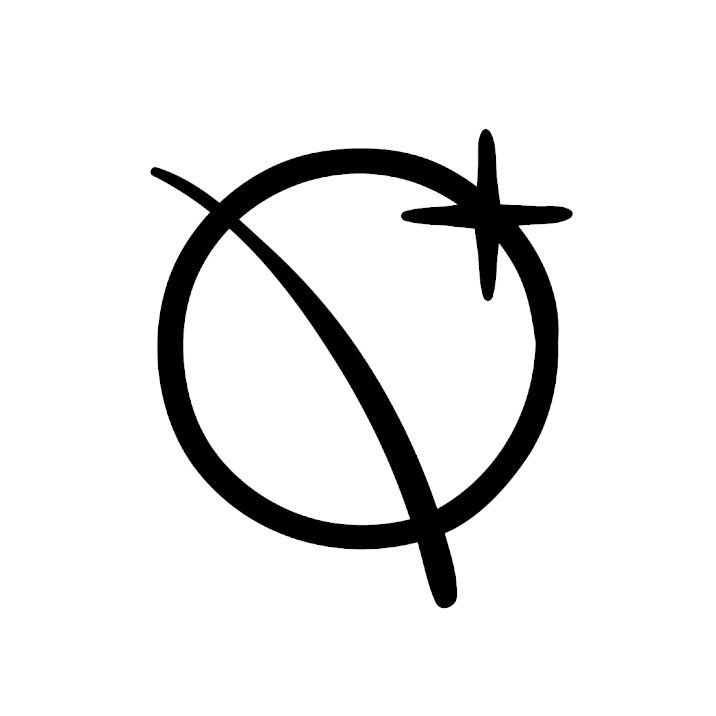
\includegraphics[height=100px]{ywf.png}

\end{minipage}

\end{document}
